

The PAK/PPK protocols were first introduced by Boyko, MacKenzie and Patel in~\cite{BoMaPa00} in 2000
as a Diffie-Hellman based provably secure PAKEs. The PAK protocol contained explicit key confirmation
while PPK did not. An augmented version of it, namely PAK-X, was also introduced in the same paper.

The setting of PAK/PPK is similar to all other Diffie-Hellman based PAKEs. What is different is its dependencies on perfect hash functions.

Let $\pi$ be the password. Let $p, q$ be large primes and $p = rq+1$, where $r, q$ are relatively prime.
Let $g$ be a generatorof a subgroup of $\mathbb{Z}^\ast_p$ of size $q$ where the Decision
 Diffie-Hellman(DDH) problemis infeasible. Let $H_1, H_{2a}, H_{2b}, H_3$ be independent random hash 
functions. The PAK and PPKprotocols are described as in Figures \ref{fig:pak} and \ref{fig:ppk}. \comment{Yi: Any idea what's going on here?}

\begin{figure}[h]
    \centering
    \label{fig:pak}
    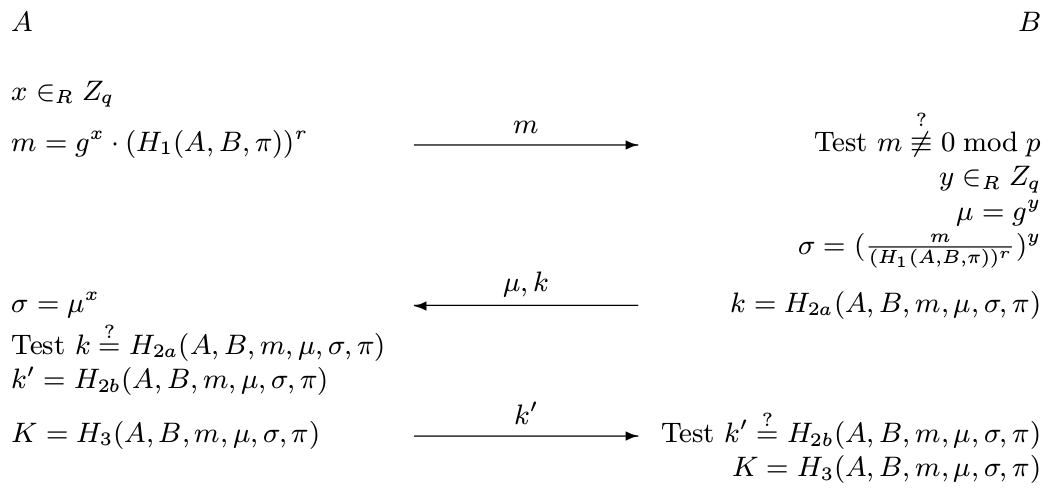
\includegraphics[scale=0.4]{pak_protocol.png}
    \caption{The PAK protocol.}
\end{figure}

\begin{figure}[h]
    \centering
    \label{fig:ppk}
    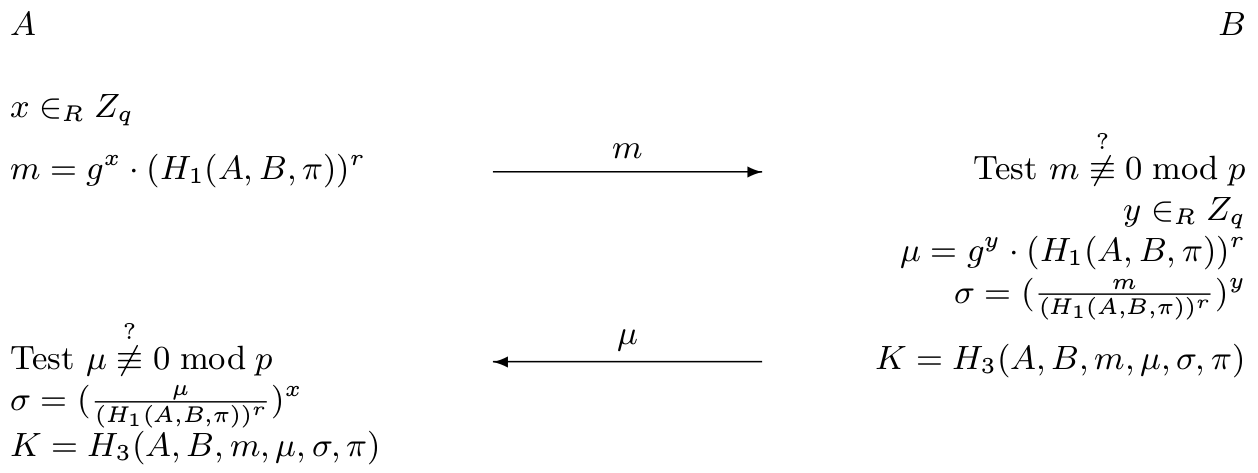
\includegraphics[scale=0.33]{ppk_protocol.png}
    \caption{The PPK protocol.}
\end{figure}

As for the security of the protocols, Boyko, MacKenzie and Patel has developed a new formal model for
 PAKEs in~\cite{BoMaPa00}, with which they have proved that PAK is secure in the random oracle model 
and PPK is secure in the implicit-authentication model, provided DDH is intractable. The newly proposed 
model and definition of security does not correspond directly to the four properties mentioned earlier in this section. However, it can be extrapolated from the proof that under the appropriate model and 
assumptions, the protocols are indeed able to provide forward secrecy as well as secure against online 
and offline dictionary attacks.












